\chapter{Experimental Results}

\section{Technical Aproach}

In order to evaluate the suitability of advanced light transport algorithms to heterogeneous systems, there were developed optimized implementations of all algorithms for both \gls{cpu} and \gls{gpu}. These implementations were developed using specialized ray tracing libraries, namely Nvidia Optix \citep{parker2010optix} and Intel Embree \citep{wald2014embree}.

Integrating both \gls{cpu} and \gls{gpu} implementations using DICE was simple, although some adaptations were applied in order to improve efficiency. DICE considers every \gls{cpu} core as an independant device, the same way it considers a \gls{gpu} for the purpose of work sharing. However, for photon mapping based algorithms this is innapropriate because if image plane division was applied, it would force communication between the \gls{cpu} and the \gls{gpu} in every iteration. If an iteration division was applied, for every \gls{cpu} core a complete photon map would be stored in the main memory. In order to solve these issues, DICE was configured to consider all the \gls{cpu} cores as a monolithic device, leaving the distribution of work in the \gls{cpu} to the application code. The work between the \gls{cpu} and the \gls{gpu} is then distributed in a set of independent iterations, eliminationg all communication needs. Between the \gls{cpu} cores the image plane is divided, eliminating the excesive memory use.

\section{Methodology}

In order to test the scalability and efficiency of the studied algorithms, the execution times of the studied algorithms were measured using only the \gls{gpu}, and while using only the \gls{cpu} or both, with a varying number of \gls{cpu} cores and threads per core, in order to evaluate the gain of using \gls{ht}. The workload distribution between the devices was also measured by the DICE scheduler. Every time measurement was executed five times, selecting the best time as the final result. These tests were executed using the Living Room Scene with a resolution of 1024x768 and 50 samples per pixel.

In order to evaluate the image quality produced by the studied algorithms, three scenes were used for testing, each with a different goal. The Sponza scene, courtesy of Crytek, is an outdoor scene with only diffuse materials, but complex geometry nonetheless. The Kitchen scene from Lux Renderer, is an indoor scene with glossy materials. The final and most complex scene, the Living Room, courtesy of Iliyan Georgiev, is an indoor scene as well but with an emphasis on reflected caustics and complex lighting. For every scene a reference image was rendered with \gls{vcm} with 100000 samples per pixel. Then for every algorithm a set of images with an approximate rendering time were produced. All these images were compared to the reference image using the \gls{rmse} metric.

\begin{figure}[h]
\centering
\begin{minipage}[b]{0.3\linewidth}
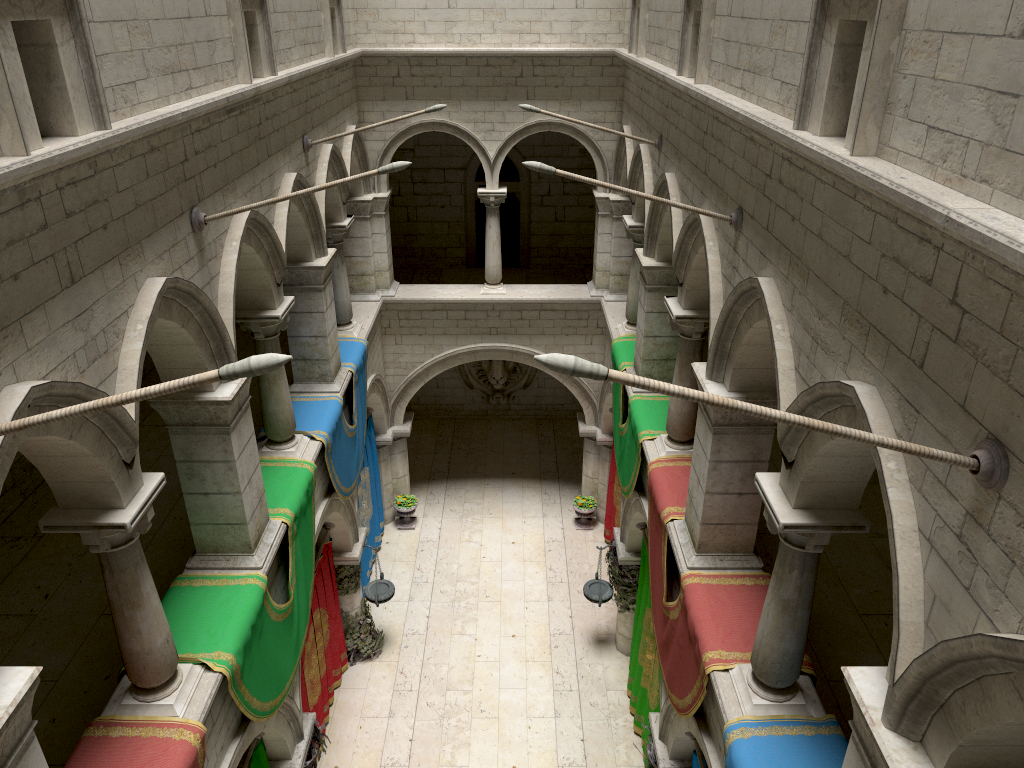
\includegraphics[width=\linewidth]{img/sponza_ref.jpg}
\caption{\label{img:sponza_ref} Sponza scene reference image.}
\end{minipage}
\quad
\begin{minipage}[b]{0.3\linewidth}
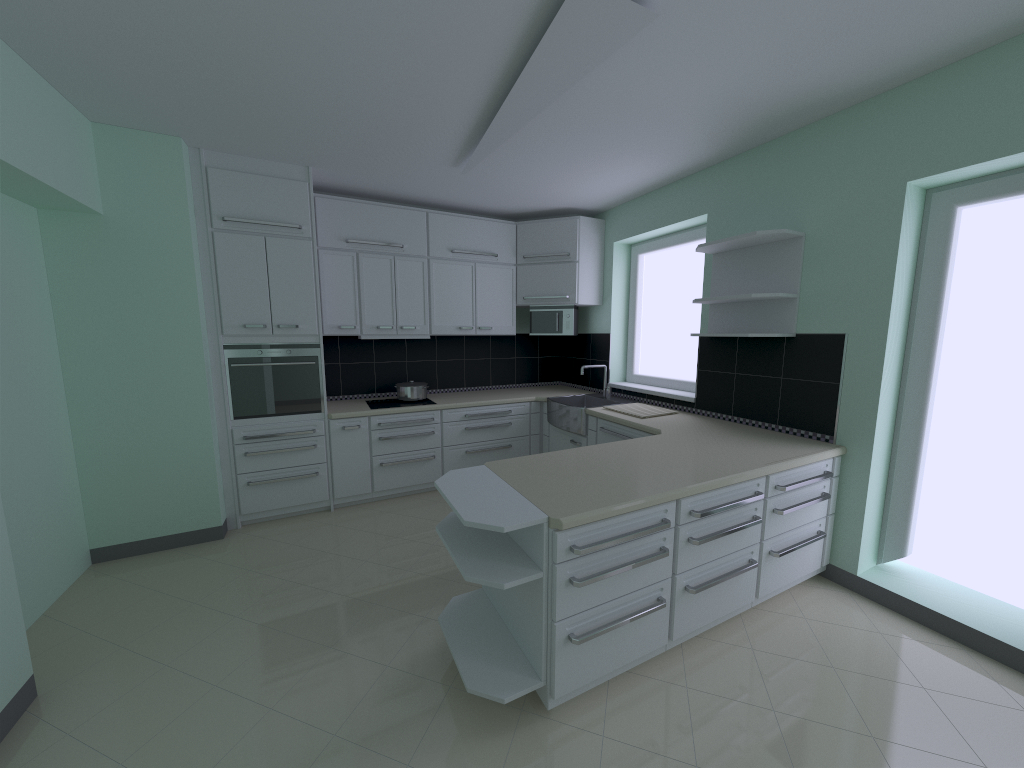
\includegraphics[width=\linewidth]{img/kitchen_ref.jpg}
\caption{\label{img:kitchen_ref} Kitchen scene reference image.}
\end{minipage}
\quad
\begin{minipage}[b]{0.3\linewidth}
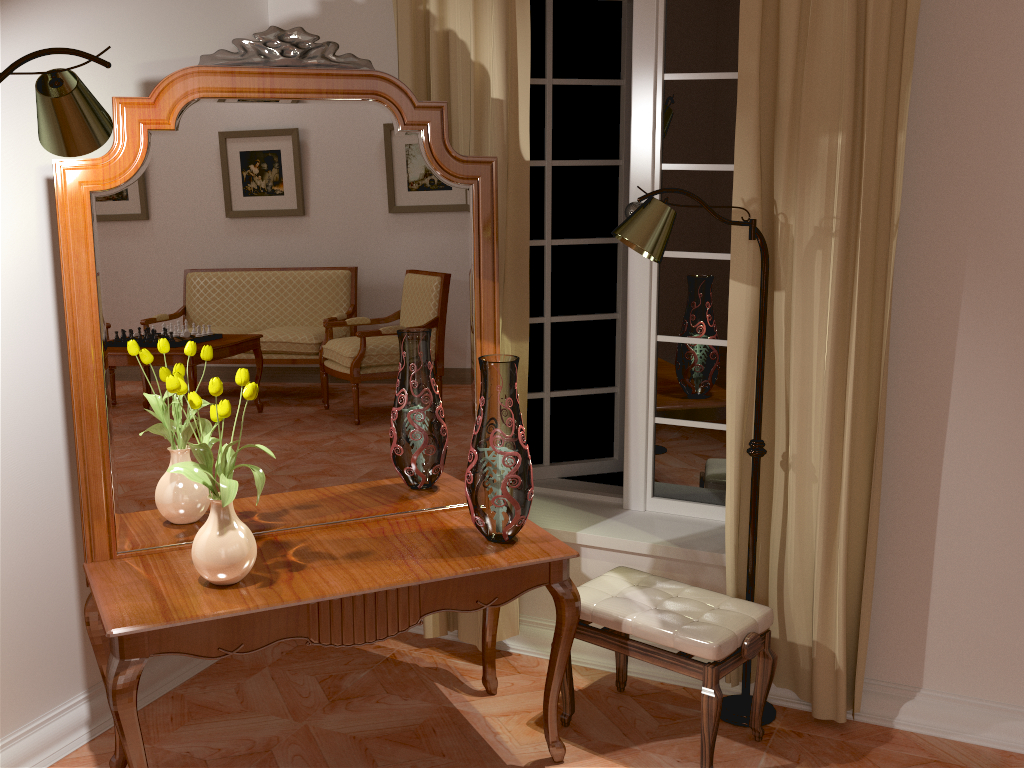
\includegraphics[width=\linewidth]{img/livingroom_ref.jpg}
\caption{\label{img:livingroom_ref} Living Room scene reference image.}
\end{minipage}

\end{figure}

\section{Experimental Setup}

All experiments were executed on a dual-socket computer with two 10 core Intel Xeon E5-2670 v2 \gls{cpu} at the frequency of 2.50GHz, 64 GB of RAM and a Nvidia Tesla K20 \gls{gpu}.

Every software used was updated to the versions listed in table~\ref{tab:soft_ver}.

\begin{table}[h]
\centering
\begin{tabular}{|l|l|}

\hline
Software & Version \\
\hline
Linux & 2.6.32-279 \\
\hline
GCC & 4.8.2 \\
\hline
CUDA Toolkit & 5.5 \\
\hline
Optix & 3.7 \\
\hline
Embree & 2.5.1 \\
\hline

\end{tabular}
\caption{\label{tab:soft_ver} Software Versions Used}
\end{table}

\section{Result Analisys}

\subsection{Excution Time Results}

\begin{figure}[H]
\centering
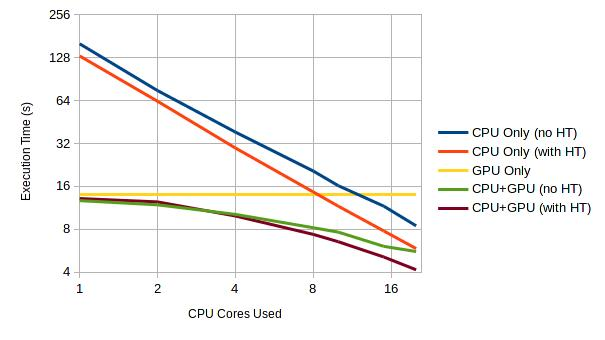
\includegraphics[width=0.8\linewidth]{img/ptTexec.jpg}
\caption{\label{img:ptTexec} Path Tracer Execution Times}
\end{figure}

\begin{figure}[H]
\centering
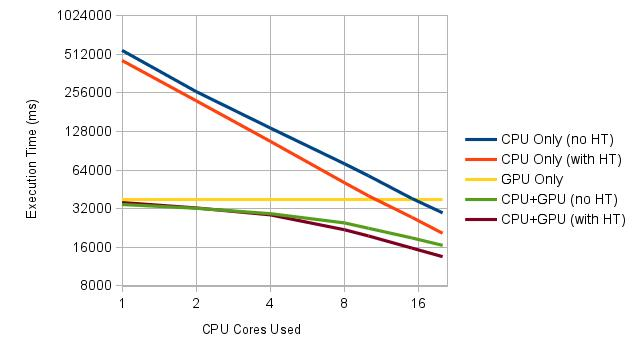
\includegraphics[width=0.8\linewidth]{img/bptTexec.jpg}
\caption{\label{img:bptTexec} Bidirectional Path Tracer Execution Times}
\end{figure}

\begin{figure}[H]
\centering
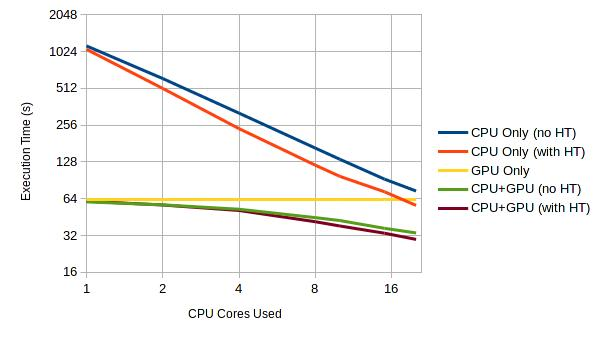
\includegraphics[width=0.8\linewidth]{img/bpmTexec.jpg}
\caption{\label{img:bpmTexec} Bidirectional Photon Mapping Execution Times}
\end{figure}

\begin{figure}[H]
\centering
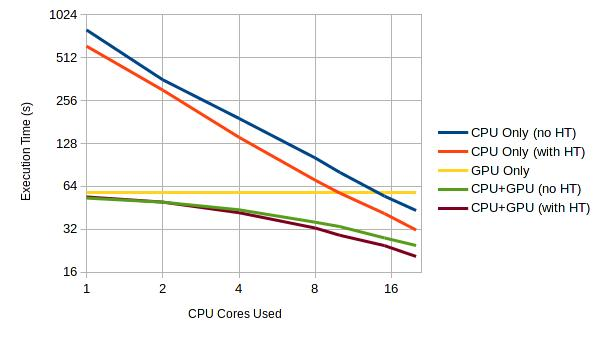
\includegraphics[width=0.8\linewidth]{img/vcmTexec.jpg}
\caption{\label{img:vcmTexec} VCM Execution Times}
\end{figure}

All the execution times measured indicate that all the algorithms studied are scalable and take advantage of both devices in the rendering process.

\subsection{CPU Speedup Results}

\begin{figure}[H]
\centering
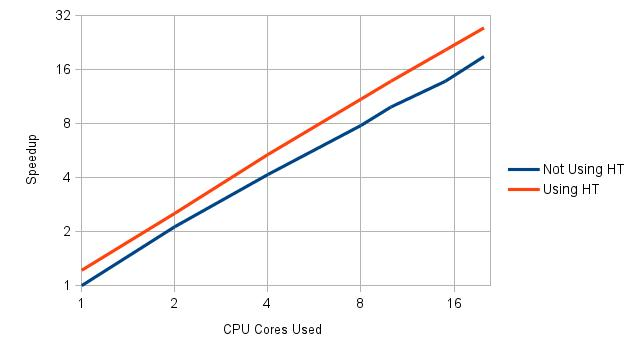
\includegraphics[width=0.8\linewidth]{img/ptSpeedup.jpg}
\caption{\label{img:ptSpeedup} Path Tracer Speedup}
\end{figure}

\begin{figure}[H]
\centering
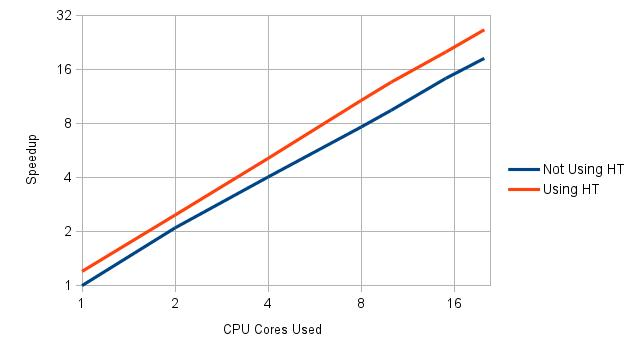
\includegraphics[width=0.8\linewidth]{img/bptSpeedup.jpg}
\caption{\label{img:bptSpeedup} Bidirectional Path Tracer Speedup}
\end{figure}

\begin{figure}[H]
\centering
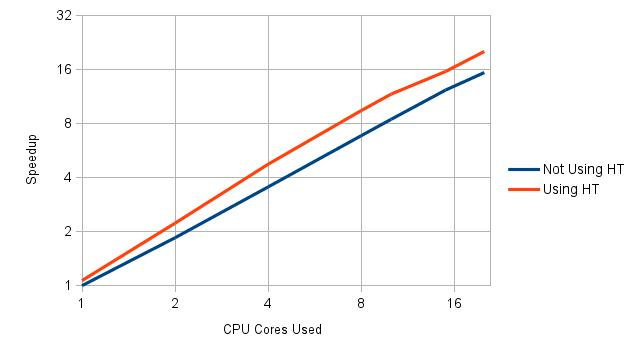
\includegraphics[width=0.8\linewidth]{img/bpmSpeedup.jpg}
\caption{\label{img:bpmSpeedup} Bidirectional Photon Mapping Speedup}
\end{figure}

\begin{figure}[H]
\centering
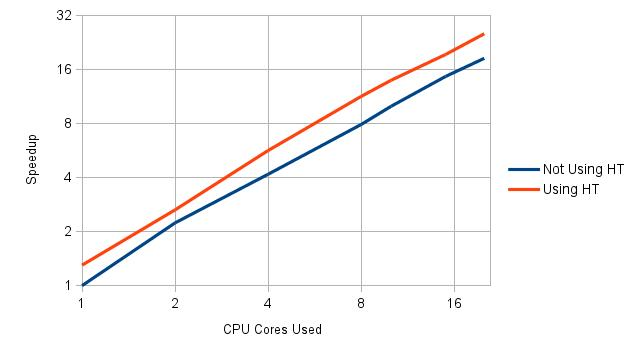
\includegraphics[width=0.8\linewidth]{img/vcmSpeedup.jpg}
\caption{\label{img:vcmSpeedup} VCM Speedup}
\end{figure}

Every algorithm except Bidirectional Photon Mapping achieve an almost linear speedup, while this only achives a speedup of 15.4 using 20 cores. All algorithms seem to take advantage of Hyper Threading, which increases the overall performance between 30\% to 50\%.

\subsection{CPU Parallelization Eficiency Results}

\begin{figure}[H]
\centering
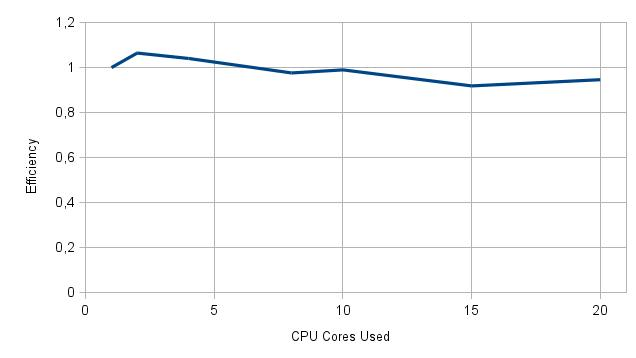
\includegraphics[width=0.8\linewidth]{img/ptEff.jpg}
\caption{\label{img:ptEff} Path Tracer Efficiency}
\end{figure}

\begin{figure}[H]
\centering
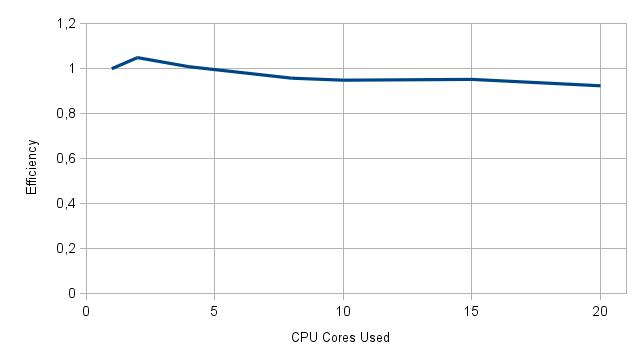
\includegraphics[width=0.8\linewidth]{img/bptEff.jpg}
\caption{\label{img:bptEff} Bidirectional Path Tracer Efficiency}
\end{figure}

\begin{figure}[H]
\centering
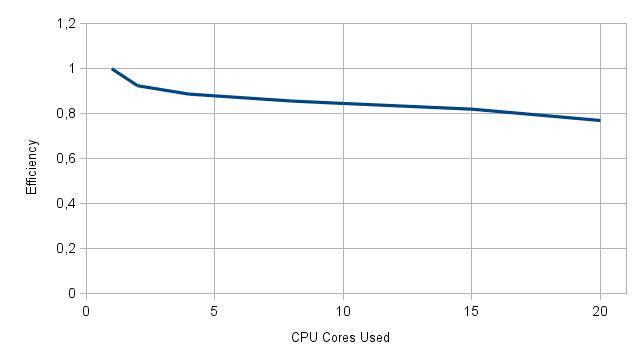
\includegraphics[width=0.8\linewidth]{img/bpmEff.jpg}
\caption{\label{img:bpmEff} Bidirectional Photon Mapping Efficiency}
\end{figure}

\begin{figure}[H]
\centering
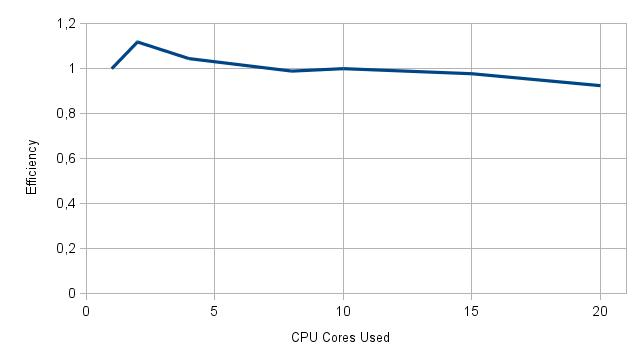
\includegraphics[width=0.8\linewidth]{img/vcmEff.jpg}
\caption{\label{img:vcmEff} VCM Efficiency}
\end{figure}

Every algorithms except Bidirectional Photon Mapping has a parallelization efficiency above 0.9, while this falls to an efficiency of 0.77 using 20 cores. This inefficiency may be due to the high memory access this algorithm has compared to all the other algorithms.

\subsection{Workload Distribution Results}

\begin{figure}[H]
\centering
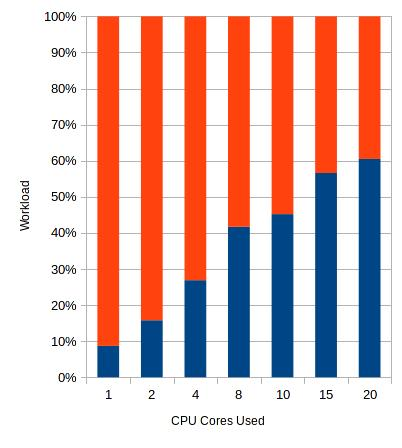
\includegraphics[width=0.8\linewidth]{img/ptwl.jpg}
\caption{\label{img:ptwl} Path Tracer Workload Distribution}
\end{figure}

\begin{figure}[H]
\centering
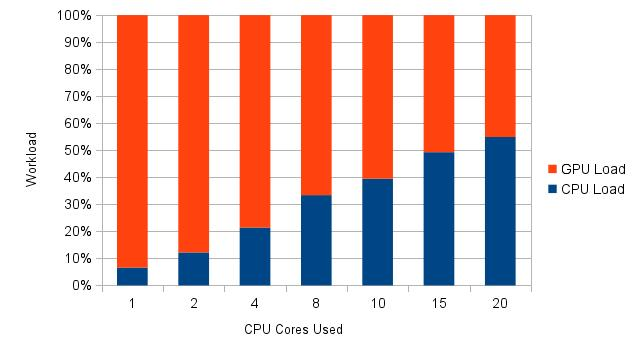
\includegraphics[width=0.8\linewidth]{img/bptwl.jpg}
\caption{\label{img:bptwl} Bidirectional Path Tracer Workload Distribution}
\end{figure}

\begin{figure}[H]
\centering
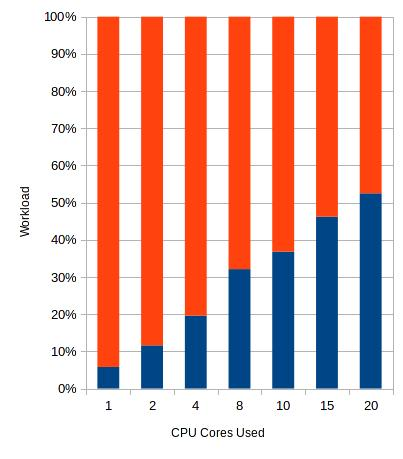
\includegraphics[width=0.8\linewidth]{img/bpmwl.jpg}
\caption{\label{img:bpmwl} Bidirectional Photon Mapping Workload Distribution}
\end{figure}

\begin{figure}[H]
\centering
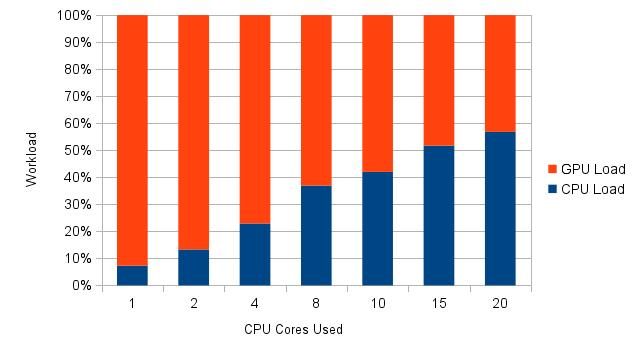
\includegraphics[width=0.8\linewidth]{img/vcmwl.jpg}
\caption{\label{img:vcmwl} VCM Workload Distribution}
\end{figure}

\subsection{Image Quality Results}

\begin{figure}[H]
\centering
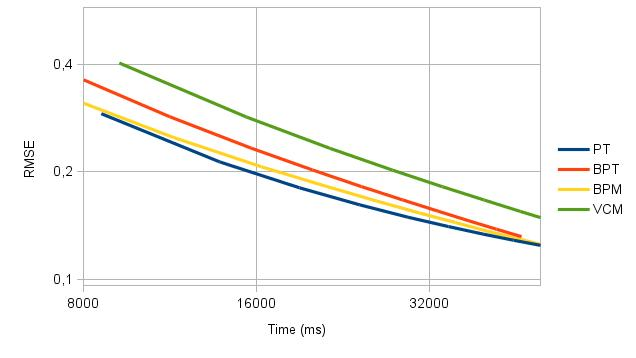
\includegraphics[width=0.8\linewidth]{img/sponzaImgq.jpg}
\caption{\label{img:sponzaImgq} Sponza Image Quality}
\end{figure}

\begin{figure}[H]
\centering
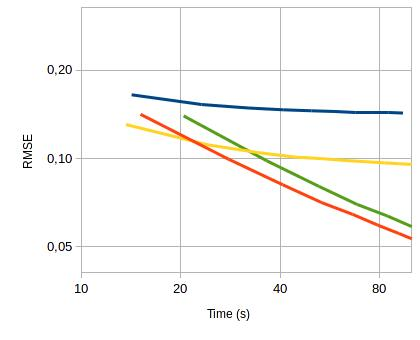
\includegraphics[width=0.8\linewidth]{img/kitchenImgq.jpg}
\caption{\label{img:kitchenImgq} Kitchen Image Quality}
\end{figure}

\begin{figure}[H]
\centering
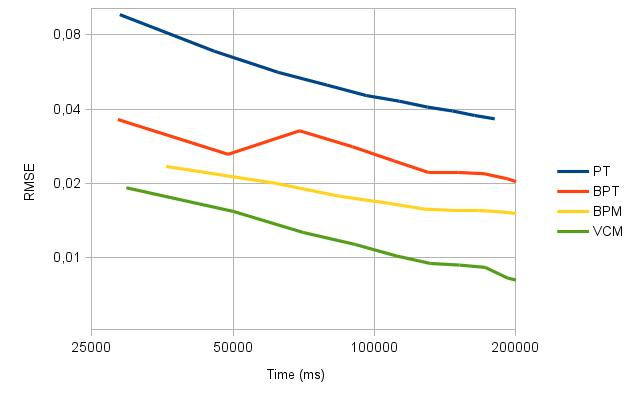
\includegraphics[width=0.8\linewidth]{img/livingroomImgq.jpg}
\caption{\label{img:livingroomImgq} Livingroom Image Quality}
\end{figure}

In the Sponza scene, all algorithms seem to converge to the right solution, however Path Tracing is the best algorithms in this case. This may be due to the outdoor scene configuration where many of the light paths traced are lost and miss the scene, as well as the simple material lighting which is completely captured by Path Tracing, not needing more complex solutions.

In the Kithcen scene, both Bidirectional Path Tracer and Vertex Connecion and Merging algorithms converge to the expected result, although the former is faster for this scene. Both Path tracer and Bidirectional Photon Mapping present lower convergence rates due to the high variance of the lighting effects present, namely caustics incident on glossy surfaces.

In the Living Room scene, Vertex Connection and Merging has the fastest convergence, while the remaining algorithms converges much more slowly.